\documentclass[12pt,a4paper]{scrbook}
\usepackage[ngerman]{babel}
\usepackage{amsmath}
\usepackage{booktabs}
\usepackage{coffee4}
\usepackage{color}
\usepackage{epsfig}
\usepackage{eso-pic}
\usepackage{float}
\usepackage{graphicx}
\usepackage{gensymb}
\usepackage{ifthen}
\usepackage{multirow}
\usepackage{nicefrac}
%\usepackage{SIunits}
\usepackage{pstricks}
\usepackage{rotating}
\usepackage{subfig}
\usepackage{textcomp}
% Komafont modifications
\setcounter{secnumdepth}{\partnumdepth}

\usepackage[utf8]{inputenc}

\graphicspath{./pics/}
% Modified environments
\newcounter{notes}
\newenvironment{Notes}
{\begin{list} {
    \textbf{\arabic{notes}} }{\usecounter{notes}%
  \setlength{\labelsep}{0pt}%
  \setlength{\leftmargin}{0pt}%
  \setlength{\labelwidth}{0pt}%
  \setlength{\listparindent}{0pt}}}%
  {\end{list}}
\title{Kochbuch}
\author{wir}
\date{}
\begin{document}
\maketitle
\tableofcontents
\chapter{Vorspeise}
\section{Artichokes}

\begin{centering}

\end{centering}

\begin{table}[H]
  \centering
  \begin{tabular*}{1\textwidth}{rlrl}
      % &  & &  \\
& artichockes & & parmesan \\
 & parsley & & salt, pepper \\
 & garlic & & lemon juice (concentrate) \\
 & vegetable broth powder & $\nicefrac{1}{2}$-1 large glasses & white wine \\
\end{tabular*}
\end{table}

%Zubereitung:
\begin{Notes}
\item Cut off stem of the artichockes, keep $\nicefrac{1}{4}$ of the stem. Tear away the outermost leafs of the artichockes and slacken them (pull leaves apart lightly).
\item Place artichocks in a large pot with water and lemon juice.
\item For the paste: Combine olive oil with chopped parsley, garlic, parmesan, salt and pepper.
\item Take artichocks out of the pot and allow the excess water to drip off. Fill with paste and press in small additional dice of parmesan.
\item Lay artichocks and the saved $\nicefrac{1}{4}$ stems in a large pot and fill up with water until half covered. Add 2-3\,ts vegetable broth powder and boil until the water is reduced to about $\nicefrac{1}{4}$.
\item Now add $\nicefrac{1}{2}$-1 large glasses of white wine and let boil a little more.
  \item The artichockes are done, when the leafes can be pulled off easily and the pulp can easily be pulled off with your teeth.
\end{Notes}
\vfill
\begin{figure}[H]
  \centering
  \includegraphics[width=0.5\textwidth]{artischocken.jpg}
\end{figure}
\newpage

\section*{Artischocken}

\begin{centering}

\end{centering}

\begin{table}[H]
  \centering
    
  \begin{tabular*}{1\textwidth}{rlrl}
      % &  & &  \\
 & Artischocken & & Parmesan \\
 & Petersilie & & Salz, Pfeffer \\
 & Knoblauch & & Zitronensaft(konzentrat) \\
 & Gemüsebrühe & $\nicefrac{1}{2}$-1 große Gläser & Weißwein \\
  \end{tabular*}
\end{table}

%Zubereitung:
\begin{Notes}
\item Stiel der Artischocke abschneiden, $\nicefrac{1}{4}$ des Stiels behalten. Äußerste Blätter der Artischocken abreißen, Artischocken lockern (die Blätter leicht auseinander ziehen).
\item Artischocken in einem großen Topf mit Wasser und Zitronensaft einlegen.
\item Für die Paste: Olivenöl mit Petersilie, Knoblauch, Parmesan, Salz und Pfeffer anrühren.
\item Die Artischocken aus dem Topf nehmen und abtropfen lassen. Artischocken mit der Paste füllen und nachträglich noch kleine Parmesanwürfel hineindrücken.
\item Artischocken und die $\nicefrac{1}{4}$-Stiele in einen großen Topf legen und mit Wasser füllen bis sie zur Hälfte bedeckt sind. 2-3\,TL Gemüsebrühe dazu geben und kochen lassen, bis das Wasser auf ca. $\nicefrac{1}{4}$ reduziert ist.
\item Dann $\nicefrac{1}{2}$-1 große Gläser Weißwein dazu geben und noch etwas kochen lassen.
  \item Fertig sind die Artischocken, wenn man die Blätter leicht abziehen kann und das Fruchtfleisch sich ohne Mühe mit den Zähnen abziehen lässt.
\end{Notes}
\vfill
\begin{figure}[H]
  \centering
  \includegraphics[width=0.5\textwidth]{artischocken.jpg}
\end{figure}
\newpage



% Hier steht der Rezepttitel
\section{Pumpkin Soup}
% Untertitel
% Danach die Zutaten in Tabellenform
% Wie viele werden satt?

%\textbf{Zutaten:}
\begin{table}[H]
\centering
% eine Tabelle mit insgesamt 4 Spalten, falls mehr Zutaten benoetigt werden
% links: Menge, rechts: Zutat
\begin{tabular*}{1\textwidth}{rlrl}
%& && \\
2 & onions && paprika \\
21\,oz & hokkaido pumpkin & 1$\nicefrac{1}{4}$ cups & orangejuice \\
7\,oz & carrots & 3 cups &\ vegetable broth \\
2\,tbs & oil &&\\
\end{tabular*}
\end{table}
\begin{figure}[H]
  \flushright
  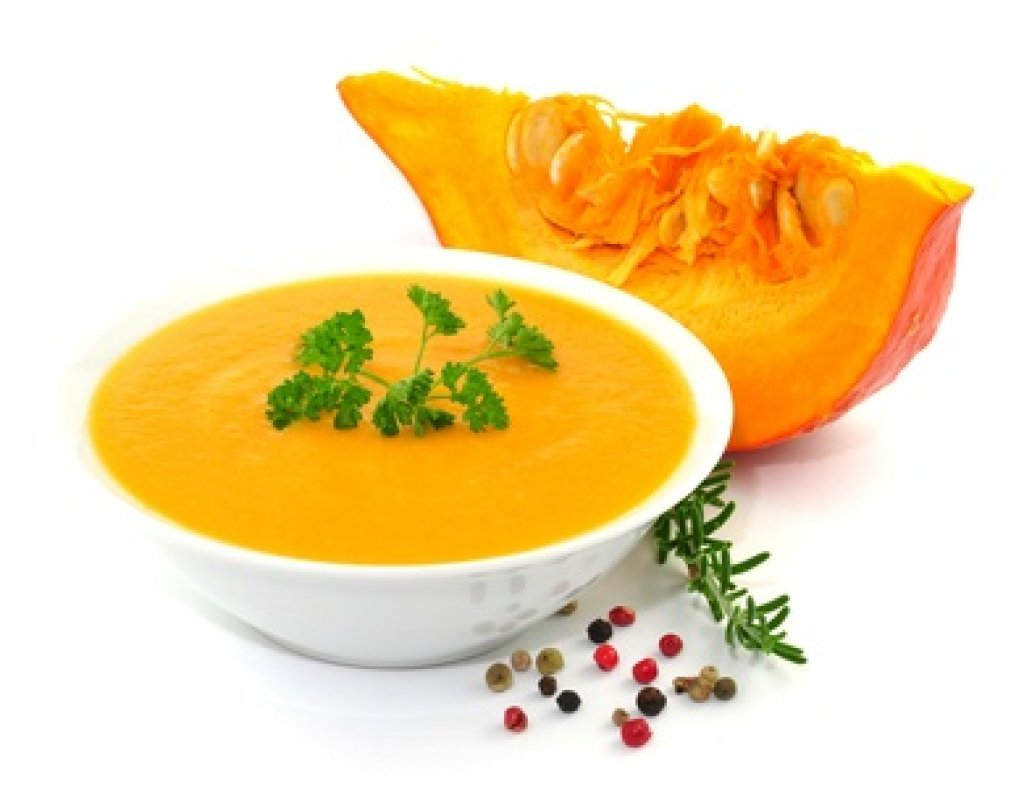
\includegraphics[width=0.35\textwidth]{kuerbissuppe.jpg}
\end{figure}
%Zubereitung:
\begin{Notes}
\item Cut pumpkin into 2\,cm sized dice, carros into slices.
\item Saut\'{e} vegetables for 5\,min in oil, season, add broth and let boil lightly for about  20\,min.
\item Afterward pur\'{e}e.
\end{Notes}
\vfill
\newpage


% Hier steht der Rezepttitel
\section*{K\"{u}rbissuppe}
% Untertitel
\begin{centering}
% Danach die Zutaten in Tabellenform
% Wie viele werden satt?
\end{centering}
%\textbf{Zutaten:}
\begin{table}[H]
\centering
% eine Tabelle mit insgesamt 4 Spalten, falls mehr Zutaten benoetigt werden
% links: Menge, rechts: Zutat
\begin{tabular*}{1\textwidth}{rlrl}
%& && \\
2 & Zwiebeln &&Paprika, edels\"{u}{\ss} \\
600\,g & Hokkaido-K\"{u}rbis & 300\,ml & Orangensaft\\
200\,g & M\"{o}hren & 700\,ml &\ Gem\"{u}sebr\"{u}he \\
2\,El & \"{O}l &&\\
\end{tabular*}
\end{table}
%Zubereitung:
\begin{Notes}
\item Hokkaido in 2\,cm gro{\ss}e W\"{u}rfel schneiden, M\"{o}hren in Scheiben.
\item Gem\"{u}se 5\,min in \"{O}l and\"{u}nsten, w\"{u}rzen, Fl\"{u}ssigkeit
dazugeben und ca. 20\,min k\"{o}cheln lassen.
\item Anschlie{\ss}end p\"{u}rieren.
\end{Notes}
\vfill
\begin{figure}[H]
  \centering
  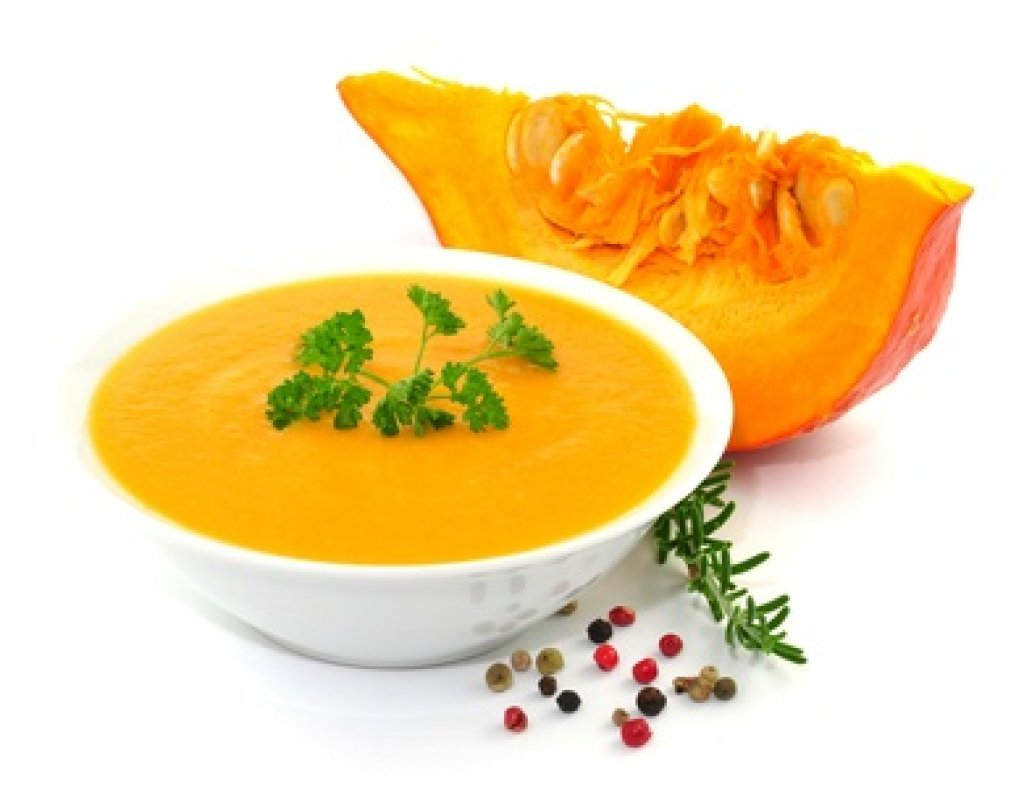
\includegraphics[width=0.75\textwidth]{kuerbissuppe.jpg}
\end{figure}


\newpage

\chapter{Hauptspeise}
\section{Fish Soup}
% Untertitel
\begin{centering}
% Danach die Zutaten in Tabellenform
% Wie viele werden satt?
For 3 hungry ones
\end{centering}
%\textbf{Zutaten:}
\begin{table}[H]
\centering
% eine Tabelle mit insgesamt 4 Spalten, falls mehr Zutaten benoetigt werden
% links: Menge, rechts: Zutat
\begin{tabular*}{1\textwidth}{rlrl}
%& && \\
3 & onions & 1.7\,cups/14\,oz & chopped tomatoes \\
2\,tbs & olive oil &3.5\,oz & zander filet\\
1 & zucchini, medium sized & 7\,oz & redfish filet\\
3 & tomatoes & 8.8\,oz & catfish filet\\
0.8 cups/6.8\,oz & fish stock && \\
&For garlic mayonaise:&&\\
& mayonaise to taste & 1 & clove of garlic\\
\end{tabular*}
\end{table}
%Zubereitung:
\begin{Notes}
\item Finely dice the onion and cut the vegetables in larger dice. Cut the fish filet in 1\,in
  pieces. 
\item Heat the olive oil in a sufficeintly large cooking pot. When hot saut\'{e}
  the onion and add the vegetables.
\item Deglaze the contents with fish fond and the chopped tomatoes and let cook
  for about 10\,min. 
\item In between chop the garlic very finely and mix with mayonaise
\item Add the fish to the rest of the soup and let steep until done. Season to taste with eg.
  rosemary or thyme. Salt and pepper and serve together with mayonaise and
  sliced baguette.
\end{Notes}
\vfill
\begin{figure}[H]
  \centering
  \reflectbox{\includegraphics[width=0.5\textwidth]{fish.jpg}}
\end{figure}
\newpage

% Hier steht der Rezepttitel
\section*{Fischsuppe}
% Untertitel
\begin{centering}
% Danach die Zutaten in Tabellenform
% Wie viele werden satt?
F\"{u}r 3 Hungrige
\end{centering}
%\textbf{Zutaten:}
\begin{table}[H]
\centering
% eine Tabelle mit insgesamt 4 Spalten, falls mehr Zutaten benoetigt werden
% links: Menge, rechts: Zutat
\begin{tabular*}{1\textwidth}{rlrl}
%& && \\
3 & Zwiebeln & 1\,Dose & gehackte Tomaten\\
2\,EL & Olivenöl &100\,g & Zanderfilet\\
1 & Zucchini, mittelgroß & 200\,g & Rotbarschfilet\\
3 & Tomaten & 250\,g & Pangasiusfilet\\
200\,ml & Fischfond && \\
&Für die Knoblauchmayonaise:&&\\
& Mayonaise nach Geschmack & 1 & Knoblauchzehe\\
\end{tabular*}
\end{table}
%Zubereitung:
\begin{Notes}
\item Die Zwiebel fein w\"{u}rfeln, das Gem\"{u}se etwas gr\"{o}ber. Den Fisch
  in ca. 2.5\,cm gro{\ss}e W\"{u}rfel schneiden. 
\item In einem ausreichend gro{\ss}en Topf das Oliven\"{o}l erhitzen und die
  Zwiebelw\"{u}rfel bei mittlerer Hitze anschwitzen. Sind die Zwiebeln glasig,
  das restliche Gem\"{u}se dazugeben und ebenfalls anbraten. 
\item Den Topfinhalt mit Fischfond und gehackten Tomaten abl\"{o}schen und
  ungef\"{a}hr 10 \,min kochen lassen. 
\item In der Zwischenzeit kann der Knoblauch sehr fein gehackt und mit der
  Mayonaise gemischt werden. 
\item Sind die 10\,min um, das Fischfilet hinzuf\"{u}gen und gar ziehen lassen.
  Nach Belieben mit z.B. Rosmarin oder Thymian w\"{u}rzen, salzen und pfeffern
  nicht vergessen!
  Zusammen mit der Mayonaise und Baguettescheiben servieren.
\end{Notes}
\vfill
\begin{figure}[H]
  \centering
  \includegraphics[width=0.5\textwidth]{fish.jpg}
\end{figure}
\newpage

% Hier steht der Rezepttitel
\section{Lasagne}
% Untertitel
\large{Flei{\ss}arbeit mit Erfolgsgarantie!}
\begin{centering}
% Danach die Zutaten in Tabellenform
% Wie viele werden satt?
F\"{u}r 6 Hungrige
\end{centering}
%\textbf{Zutaten:}
\begin{table}[H]
  \centering
    % eine Tabelle mit insgesamt 4 Spalten, falls mehr Zutaten benoetigt werden
    % links: Menge, rechts: Zutat
  \begin{tabular*}{1\textwidth}{rlrl}
    &\textbf{F\"{u}r das Ragu bolognese:}&&\\
    %&  &&  \\
    1 & M\"{o}hre & 1 Stange & Sellerie \\
    50\,g  & Pancetta & 1 & Zwiebel \\
    2 Zehen & Knoblauch &1\,EL & Butter\\
    1\,EL & Oliven\"{o}l&300\,g&gem. Hackflesich\\
    1 Dose (400\,g)&gesch\"{a}lte Tomaten & 300\,ml& Rotwein/Br\"{u}he\\
    &Salz & & schwarzer Pfeffer\\
    &&&\\

    &\textbf{F\"{u}r die Bechamelsauce:}&&\\
    50\,g & Butter & 50\,g & Mehl \\
    \nicefrac{3}{4}\,l & Milch & & Salz \\
    &schwarzer Pfeffer& & geriebene Muskatnuss\\
    &&&\\
    &\textbf{Zum Einschichten:}&&\\
    250\,g & Nudelplatten & & Salz\\
    250\,g & Mozzarella & 100\,g & frisch geriebener Parmesan\\
    1\,EL & Butter
  \end{tabular*}
\end{table}

%Zubereitung:
\begin{Notes}
  \item F\"{u}r die Bolognese (die genauso gekocht wird, wenn man sie zu
    Spaghetti essen will) M\"{o}hre sch\"{a}len, Sellerie waschen, beides ganz
    fein w\"{u}rfeln. Pancetta ebenfalls in W\"{u}rfelchen schneiden, Zwiebel
    und Knoblauch nach dem Sch\"{a}len auch.

  \item Butter und \"{O}l in der Pfanne oder im Topf warm werden lassen.
    Pancetta, Gem\"{u}se, Zwiebel und Knoblauch dazur\"{u}hren und
    and\"{u}nsten. Hackfleisch untermischen und weitergaren bis es kr\"{u}melig
    ist. Gr\"{o}{\ss}ere Fleischst\"{u}cke dabei mit der R\"{u}ckseite vom
    Kochl\"{o}ffel auseinander dr\"{u}cken, bis sie zerfallen.
    
  \item Tomaten in der Dose klein schneiden, mit dem Wein und der Br\"{u}he
    dazusch\"{u}tten, leict salzen und pfeffern, zugedeckt bei schwacher Hitze 1
    Stunde schmurgeln lassen. Dann erst abschmecken.

  \item Jetzt zur Bechamel: Butter in einem Topf warm werden lasen, braun soll
    sie aber nicht werden. Mit dem Kochl\"{o}ffel flei{\ss}ig r\"{u}hren und das
    Mehl dazusch\"{u}tten. Weiterr\"{u}hren, bis alles glatt ausschaut. Nach und
    nach die Milch dazugie{\ss}en. Jetzt am besten mit dem Schneebesen
    r\"{u}hren, damit sich keine Kl\"{u}mpchen bilden. Sauce 10 Minuten schwach
    k\"{o}cheln lassen, mit Salz, Pfeffer und Muskat w\"{u}rzen.
    
  \item Wer sich f\"{u}r das bisschen Mehrarbeit entschieden hat: 5\,$\ell$
    Wasser mit Salz aufkochen. Nudelplatten darin 4-5\,min kochen, bis sie
    biegsam sind. Mit kaltem Wasser abscherecken.

  \item Mozzarella w\"{u}rfeln. Backofen auf 200\textdegree\,C vorheizen. Eine
    gro{\ss}e rechteckige und feuerfeste Form aus dem Schrank holen. (Die ovale
    nehmen nur Bastelfreaks.) Etwas Bechamel reingie{\ss}en. Nudelplatten drauf,
    Ragu, Bechamel, Mozzarelle und wieder Nudeln. So fortfahren, bis alles in
    der Form ist. Zum Schluss die \"{u}brige Bechamel drauf, mit Parmesan
    bestreuen und mit Butter in Fl\"{o}ckchen belegen. Ab in den Ofen damit.
    Jetzt bleiben 40\,min Zeit zum K\"{u}che aufr\"{a}umen, Tischdecken und
    Ausruhen.

\end{Notes}
So viel Zeit muss sein: gut 2 Stunden, davon 40 Minuten ganz relaxed \newline
Das schmeckt dazu: Rotwein und viel Salat
Pro Portion: 720\,kcal
%------------------------------------------------------------------------------
%----------------  English version --------------------------------------------
%------------------------------------------------------------------------------
% Hier steht der Rezepttitel
\section*{Lasagne}
% Untertitel
\large{Effort that entails success!}
\begin{centering}
% Danach die Zutaten in Tabellenform
% Wie viele werden satt?
Serves 6 hungry eaters
\end{centering}
%\textbf{Zutaten:}
\begin{table}[H]
  \centering
    % eine Tabelle mit insgesamt 4 Spalten, falls mehr Zutaten benoetigt werden
    % links: Menge, rechts: Zutat
  \begin{tabular*}{1\textwidth}{rlrl}
    &\textbf{Ragu Bolognese:}&&\\
    %&  &&  \\
    1 & carrot & 1 stick & celery \\
    1.8\,oz  & Pancetta & 1 & onion \\
    2 cloves of & garlic &1\,tbs & butter\\
    1\,tbs & olive oil & 10.5\,oz&mixed minced meat\\
    1.7\,cups/14\,oz (400\,g)&peeled tomatoes&1.25\,cups/10\,oz& red wine/vegetable broth\\
    &salt & & black pepper\\
    &&&\\

    &\textbf{Sauce Bechamel:}&&\\
    1.8\,oz & butter & 1.8\,oz & flour \\
    3.2\,cups & milk & & salt \\
    &black pepper& & ground nutmeg\\
    &&&\\
    &\textbf{To build layers:}&&\\
    8.8\,oz & pasta  & & salt\\
    8.8\,oz & mozzarella & 3.5\,oz & freshly grounded parmesan\\
    1\,tbs & butter
  \end{tabular*}
\end{table}

%Zubereitung:
\begin{Notes}
  \item For the bolognese peel the carrots and wash celery, cut into fine
    dice. (The bolognese is the same as for the spaghetti sauce). Proceed with
    the pancetta likewise and also with the garlic and the onion after having
    them peeled.
    
  \item Heat butter and oil in a pan or a pot. Stir in Pancette, vegetables,
    onion and garlic heating them up gently. Mix in minced meat and cook until
    meat crumbles. Mash larger pieces of meat with the backside of the cooking
    spoon.
  \item Cut tomatoes while still in can, pour into pot together with wine and
    broth, salt sparsely and spice with pepper, keep simmering over low heat
    for 1 hour, then spice to liking.

  \item Now the sauce bechamel: heat butter in separate pot, prevent from
    getting brown. Stir firmly while giving in the flour. Keep on stirring until
    everything looks smooth. Pour in milk bit after bit. Switch to kitchen swirl
    for stirring now, so that sauce does not get clumpsy. Simmer sauce for
    10\,min, spice with salt, black pepper and nutmeg.
  \item Who decided on the extra work: boil up 5\,$\ell$ of salted water and
    cook pasta for about 4-5\,min, until formable. Pour cold water over them.


  \item Dice mozzarella and heat up oven to 390\textdegree\,F. Get a rectangular
    fireproof oven dish out of the cupboard. Oval ones only well suited for
    DIY'ers. Cover bottom with a little sauce
    bechamel. Cover with pasta, then bolognese, bechamel, mozzarella and pasta.
    Proceed until nothing left. pour over rest of bechamel, garnish with
    parmesan and butter. Into the oven! Now 40\,min of time can be used to clean
    up the kitchen, set the table and relaxing.

\end{Notes}

Total time: about 2 hours, 40\,min easy going \newline
Acompanied well by: red wine, a lot of salad
Per serving: 720\,kcal


\section{Minestrone}

\begin{centering}

  None more often, none tastes better - To fill 4 eaters

\end{centering}

\begin{table}[H]
  \centering

  \begin{tabular*}{1\textwidth}{rlrl}
      % &  & &  \\
    4\nicefrac{1}{2} cups/17.6\,oz & mixed vegetables (best:  celery
    stalks,&&\\
    & zucchini, carrots, young savoy cabbage&&\\
    &spinach)&&\\
    1\nicefrac{1}{2}\,l & vegetable or meat broth & 4 & tomatoes\\
    7\,oz & maccaroni &1 & onion\\
    1 tin/12.7\,oz & boiled white beans & 2 cloves & garlic\\
    & salt, pepper freshly ground & 3\,tbs & olive oil \\
    4\,tbs & freshly grated parmesan\\
    &or pecorino &&\\
  \end{tabular*}
\end{table}

%Zubereitung:
\begin{Notes}
\item Clean all vegetables, peel carrots, slice vegetables in dices (celery, zucchini, carrots and tomatoes) or stripes (savoy cabbage, spinach). Peel onion and garlic and cut very fine.
\item Put a large stockpot on the stove. Let 1\,tbs oil get warm in it. Stir in onions and garlic and saut\'{e}. Add vegetable broth, mix in vegetables and let all become nice and hot.
\item The veggies has to boil lightly now for about 15\,min. Therefore turn down to medium heat. Put on the lid omly half (clamp the spoon so the lid doesn't slip).
\item Break pasta in pieces (about 5\,cm long). Rinse beans with cold water in a sieve, for the fluid is murky and slimy. Add pasta and beans to soup and let boil for about 10 more minutes, until the pasta is al dente.
\item Try the minestrone, is salt and pepper missing? Ladle soup into soup plates, sprinkle with the left oil and grated cheese and ready is the most italian soup of all times.
\end{Notes}
How much time to take: 45\,min, of which 30 are work
Goes well with: fresh white bread, toasted if you like. Also nice: A small spoon of pesto for every plate.

\begin{figure}[H]
  \centering
  \reflectbox{\includegraphics[width=0.4\textwidth]{Zucchini-Whole.jpg}}
\end{figure}
\newpage

\section*{Minestrone}

\begin{centering}

  Keine gibt's \"{o}fter, keine schmeckt besser - F\"{u}r 4 zum Sattessen

\end{centering}

\begin{table}[H]
  \centering

  \begin{tabular*}{1\textwidth}{rlrl}
      % &  & &  \\
    500\,g & gemischtes Gem\"{u}se (am besten: Stangensellerie,& &\\
    & Zucchini, M\"{o}hren, junger Wirsing,& & \\
    & Spinat)& & \\
    1\nicefrac{1}{2}\,l & Gem\"{u}se- oder Fleischbr\"{u}he & 4 & Tomaten \\
    200\,g & Maccaroni & 1 & Zwiebel\\
    1 Dose & gegarte wei{\ss}e Bohnen (360\,g) & 2 & Knoblauchzehen \\ & Salz,
    Pfeffer aus der M\"{u}hle & 3\,EL & Oliven\"{o}l\\
    4\,EL & frisch geriebener Parmesan oder Pecorino &&\\
  \end{tabular*}
\end{table}

%Zubereitung:
\begin{Notes}
\item Alles Gem\"{u}se waschen, M\"{o}hren sch\"{a}len, Gem\"{u}se in W\"{u}rfel (Sellerie, Zucchini, M\"{o}hren und Tomaten) oder Streifen (Wirsing, Spinat) schneiden. Zwiebeln und Knoblauch sch\"{a}len und ganz fein schneiden.
\item Einen gro{\ss}en Topf auf den Herd stellen. 1\,EL \"{o}l darin warm werden lassen. Zwiebeln und Knoblauch reinr\"{u}hren und anbraten. Gem\"{u}sebr\"{u}he dazugie{\ss}en, Gem\"{u}se untermischen und alles sch\"{o}n hei{\ss} werden lassen.
\item Das Gem\"{u}se soll jetzt ungef\"{a}hr 15\,min k\"{o}cheln. Also die Hitze auf mittlere Stufe stellen. Und den Deckel nur halb auflegen (Kochl\"{o}ffel dazwischen klemmen, dann rutscht der Deckel nicht).
\item Nudeln in St\"{u}cke brechen (ungef\"{a}hr 5\,cm lang). Bohnen im Sieb kalt absp\"{u}len, die Garfl\"{u}ssigkeit ist n\"{a}mlich tr\"{u}b und glibbrig. Nudeln und Bohnen zur Suppe geben und nochmal ungef\"{a}hr 10\,min weiterk\"{o}cheln lassen, bis die Nudeln al dente sind.
\item Minestrone probieren, fehlt noch Salz und Pfeffer? Suppe in tiefe Teller sch\"{o}pfen, das \"{u}brige \"{o}l dar\"{u}berlaufen lassen, K\"{a}se drauf streuen und fertig ist die italienischste Suppe aller Zeiten.
\end{Notes}

Soviel Zeit muss sein: 45\,min, davon 30 zu tun
Das schmeckt dazu: frisches Wei{\ss}brot, wer mag, kann es leicht anr\"{o}sten. Auch gut dazu: pro Teller ein L\"{o}ffelchen Pesto
\newpage

\section{Carrot Stew}
\cofeAm{1}{1}{180}{0}{0}
\begin{centering}

Serves

\end{centering}

\begin{table}[H]
  \centering
    
  \begin{tabular*}{1\textwidth}{rlrl}
      % &  & &  \\
    17.5\,oz & carrots  & 13.2\,oz & minced meat (beef) \\
	7\,oz & potatoes (optional) & & garlic flavoured salt \\
	2\,tbs & butter & & onion flavoured salt\\
	2 cups/16.9\,fl oz & (vegetable) stock & & wocester sauce \\
	2-3 sticks & leek & 1 bunch & parsley \\
	& salt, pepper &  & \\
  \end{tabular*}
\end{table}

%Zubereitung:
\begin{Notes}
\item Clean carrots/potatoes and slice into sticks. In 1\,tbs butter saut\'{e} vegetables, then add vegetable stock. Cover and let boil lightly for about 10\,min. Cut leek into rings, wash and add to the carrots. Season with salt and pepper.
\item Season minced meat with pepper, salt and garlic and onion flavoured salt. Let 1\,tbs butter melt in a pan and saut\'{e} meat. Season to taste with worcester sauce and add to the vegetables.
\item Chop parsley and serve carrot stew with parsley on top.
\end{Notes}
\vfill
\begin{figure}[H]
  \centering
  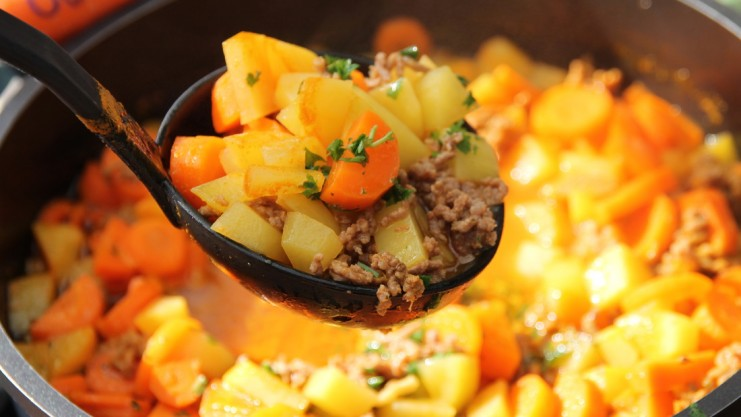
\includegraphics[width=0.65\textwidth]{moeheneintopf.jpg}
\end{figure}
\newpage

\section*{M\"{o}hreneintopf}

\begin{centering}

F\"{u}r

\end{centering}

\begin{table}[H]
  \centering
    
  \begin{tabular*}{1\textwidth}{rlrl}
      % &  & &  \\
    500\,g & M\"{o}hren  & 375\,g & (Rinder-)Hackfleisch \\
	200\,g & Kartoffeln (optional) & & Knoblauchsalz \\
	2\,EL & Butter & & Zwiebelsalz \\
	\nicefrac{1}{2}\,l & Br\"{u}he &  & Wocestersauce \\
	2-3 Stangen & Lauch & 1 Bd.& Petersilie \\
	& Salz, Pfeffer &  & \\
  \end{tabular*}
\end{table}

%Zubereitung:
\begin{Notes}
\item Die M\"{o}hren/Kartoffeln waschen, putzen und in Stifte schneiden, in 1\,EL Butter kurz and\"{u}nsten und mit der Br\"{u}he auff\"{u}llen. Zugedeckt etwa 10\,min k\"{o}cheln lassen. Den Lauch in Ringe schneiden, waschen und hinzuf\"{u}gen, mit Salz und Pfeffer w\"{u}rzen.
\item Rinderhack mit Pfeffer, Salz und, nach Geschmack, mit Knoblauch- und Zwiebelsalz w\"{u}rzen und in einer Pfanne mit 1\,EL Butter anbraten. Mit Worcestersauce w\"{u}rzen und zu dem Gem\"{u}se geben.
\item Petersilie hacken und Eintopf mit Petersilie bestreut servieren.
\end{Notes}
\vfill
\begin{figure}[H]
  \centering
  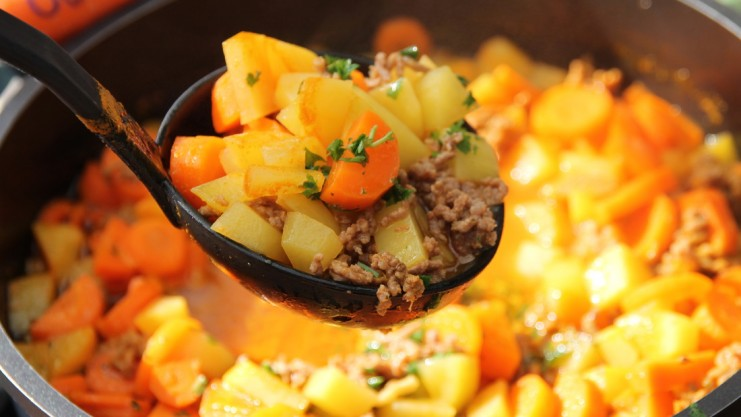
\includegraphics[width=0.65\textwidth]{moeheneintopf.jpg}
\end{figure}
\newpage

% Hier steht der Rezepttitel
\section{Oma's K\"{o}nigsberger Meatballs}
% Untertitel
\begin{centering}
% Danach die Zutaten in Tabellenform
% Wie viele werden satt?
Serves 10
%\textbf{Zutaten:}
\begin{table}[H]
\centering
% eine Tabelle mit insgesamt 4 Spalten, falls mehr Zutaten benoetigt werden
% links: Menge, rechts: Zutat
\begin{tabular*}{1\textwidth}{rlrl}
%& && \\
35\,oz & ground meat & & lemon juice \\
1$\nicefrac{1}{2}$ & bread rolls & 14.1\,oz / 1$\nicefrac{1}{2}$ cups & sour cream \\
14.1\,oz / 1$\nicefrac{1}{2}$ cups & cr\`{e}me fra\^{i}che &3.5-5\,oz / $\nicefrac{3}{4}$ cup & capers \\
&milk to soak &2x &white gravy powder\\
2-3 & onions & &butter\\
2 & eggs & 35\,oz / 1\,$\ell$ & vegetable broth\\
\end{tabular*}
\end{table}
\end{centering}
%Zubereitung:
\begin{Notes}
\item The night before, soak the bread rolls in milk, thoroughly squeeze out the milk.
\item Cut onions into dices and saut\'{e} onions until transparent, then add the minced meat. Combine and blend with pepper, salt, 2 eggs and bread rolls. 
\item Form meatballs and let steep in vegetable broth for 20\,min.
\item Remove meatballs and stir the white gravy powder into the broth. Add sour cream and cr\`{e}me fra\^{i}che. Together with meatballs and capers once more bring to a boil.
\end{Notes}

% Hier steht der Rezepttitel
\section*{Omas K\"{o}nigsberger Klopse}
% Untertitel
\begin{centering}
% Danach die Zutaten in Tabellenform
% Wie viele werden satt?
F\"{u}r 10 Hungrige
%\textbf{Zutaten:}
\begin{table}[H]
\centering
% eine Tabelle mit insgesamt 4 Spalten, falls mehr Zutaten benoetigt werden
% links: Menge, rechts: Zutat
\begin{tabular*}{1\textwidth}{rlrl}
%& && \\
1\,kg & Hackflesich &&Zitronensaft \\
1\nicefrac{1}{2} & Br\"{o}tchen & 2 Becher & Saure Sahne\\
2 Becher & Cr\`{e}me fra\^{i}che &100-150\,g&Kapern\\
&Milch zum Einweichen &2x &helle So{\ss}e (Fertigprodukt)\\
2-3 & Zwiebeln & &Butter\\
2 & Eier & 1\,$\ell$ & Gem\"{u}sebr\"{u}he\\
\end{tabular*}
\end{table}
\end{centering}
%Zubereitung:
\begin{Notes}
\item Am Vorabend Br\"{o}tchen in Milch einweichen, kr\"{a}ftig ausdr\"{u}cken.
\item Zwiebeln w\"{u}rfeln und glasig anbraten, Hackfleisch dazugeben. Mit
Pfeffer, Salz, 2 Eiern, und Br\"{o}tchen durchmengen.
\item Klopse aus der Masse formen und in Gem\"{u}sebr\"{u}he 20\,min ziehen
lassen.
\item Klopse entfernen und die helle So{\ss}e in der Br\"{u}he anr\"{u}hren.
Saure Sahne und Cr\`{e}me fra\^{i}che dazugeben und mit den Klopsen,
zusammen mit den Kapern, aufkochen.
\end{Notes}

\section{Zucchini Stew}

\begin{centering}

Serves 4.

\end{centering}

\begin{table}[H]
  \centering
    
  \begin{tabular*}{1\textwidth}{rlrl}
      % &  & &  \\
125-150\,g & ground meat & 2 & eggs \\
3 & zucchini & 200-300\,g & spaghetti \\
4 & potatoes & & vegetable broth \\
1 & small onion & & parmesan \\
 & olive oil & & \\
\end{tabular*}
\end{table}

%Zubereitung:
\begin{Notes}
\item Cut onion, zucchini, and potatoes into dice. Roest ground meat and onion in a pot with olive oil. Add zucchini and potoatoes and saut\'{e}.

\item Cover with water. Add 2\,ts vegetable broth and season with salt and pepper. Break spaghetti into pieces and add to the soup. Whisk eggs lightly and stir in ground parmesan.

\item Shortly before the spaghetti are done, add whisked eggs and let steep for 5-10 more minutes.
\end{Notes}


\section*{Zucchinieintopf}

\begin{centering}

F\"{u}r 4 Personen.

\end{centering}

\begin{table}[H]
  \centering
    
  \begin{tabular*}{1\textwidth}{rlrl}
      % &  & &  \\
125-150\,g & Hackfleisch & 2 & Eier \\
3 & Zucchini & 200-300\,g & Spaghetti \\
4 & Kartoffeln & & Gemüsebrühe \\
1 & kleine Zwiebel & & Parmesan \\
  \end{tabular*}
\end{table}

%Zubereitung:
\begin{Notes}
\item Zwiebel, Zucchini und Kartoffeln würfeln. Hackfleich mit Zwiebeln in einem Topf in Olivenöl anbraten. Zucchinis und Kartoffeln dazugeben und andünsten.

\item Alles mit Wasser bedecken. 2\,TL Gemüse Brühe dazu geben und mit Salz und Pfeffer abschmecken. Spaghetti klein machen und und in den Topf geben. Zwei Eier verschlagen und gerieben Parmesan unterrühren.

\item Kurz bevor die Nudeln fertig sind, die verschlagen Eier dazu geben und das ganze noch 5-10\,min ziehen lassen. 
\end{Notes}



  \chapter{Dessert}
% Hier steht der Rezepttitel
\section{lecker Rezept}

% Danach die Zutaten in Tabellenform
% Wie viele werden satt?
F\"{u}r 10 Hungrige
%\textbf{Zutaten:}
\begin{table}[H]\label{tab:am_s_k}
  \centering
    % eine Tabelle mit insgesamt 4 Spalten, falls mehr Zutaten benoetigt werden
    % links: Menge, rechts: Zutat
  \begin{tabular*}{1\textwidth}{rlrl}
      %&  &&  \\
    100\,g & Zucker  &3&Eier \\
  \end{tabular*}
\end{table}

%Zubereitung:

Lorem Ipsum dolor sit amet\ldots






% Hier steht der Rezepttitel
\section{Dulce di Leche Creme}
% Untertitel
% Danach die Zutaten in Tabellenform
% Wie viele werden satt?
\begin{minipage}{0.45\textwidth}
  \flushleft
  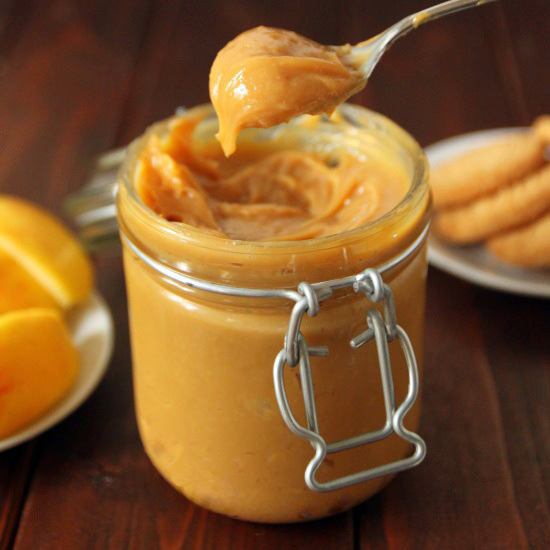
\includegraphics[width=0.7\textwidth]{dulce.jpg}
\end{minipage}
\begin{minipage}{0.55\textwidth}
Yields about 1$\nicefrac{3}{4}$-2 cups of sweet cream.
%\textbf{Zutaten:}
\begin{table}[H]
\centering
% eine Tabelle mit insgesamt 4 Spalten, falls mehr Zutaten benoetigt werden
% links: Menge, rechts: Zutat
\begin{tabular*}{1\textwidth}{rlrl}
%& && \\
3 cups  & whole milk & 1 cup & sugar \\
1$\nicefrac{1}{2}$ cups & cream & 2 pinches & salt \\
\end{tabular*}
\end{table}
\end{minipage}
%Zubereitung:
\begin{Notes}
\item Mix all ingredients in a pot and bring to a boil uncovered. Stirring constantly, let boil lighlty until thickend to desired consistency (creamy) and the color turns golden. Watch out, it's going to get even more firm when it cools down!
\item Tip: Reducing to about $\nicefrac{1}{3}$ of the initial volume is a good rule of thumb. In these quantities this will take about one hour, during which the pot cannot stay unobserved.
\item Store in the fridge.
\end{Notes}
\newpage
% Hier steht der Rezepttitel
\section*{Dulce di Leche-Creme}
% Untertitel
% Danach die Zutaten in Tabellenform
% Wie viele werden satt?
\begin{minipage}{0.55\textwidth}
Für etwa 400\,ml süße Creme
%\textbf{Zutaten:}
\begin{table}[H]
\centering
% eine Tabelle mit insgesamt 4 Spalten, falls mehr Zutaten benoetigt werden
% links: Menge, rechts: Zutat
\begin{tabular*}{1\textwidth}{rlrl}
%& && \\
800\,ml & Vollmilch & 200\,g & Zucker \\
400\,ml & Sahne & 2 Prisen & Salz \\
\end{tabular*}
\end{table}
\end{minipage}
\begin{minipage}{0.45\textwidth}
  \flushright
  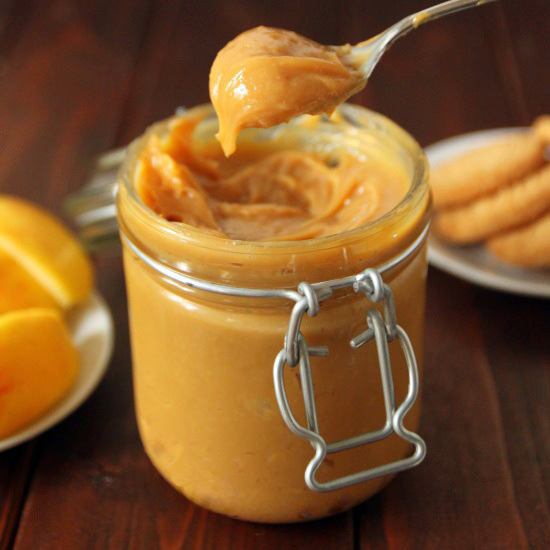
\includegraphics[width=0.7\textwidth]{dulce.jpg}
\end{minipage}
%Zubereitung:
\begin{Notes}
\item Alle Zutaten ohne Deckel in einem Topf zum Kochen bringen. Unter Rühren köcheln lassen, bis es auf die gewünschte Konsistenz (cremig) und Farbe (goldgelb) eingekocht ist. Achtung, es wird noch fester, wenn es abkühlt! 
\item Tipp: Auf etwa $\nicefrac{1}{3}$ der Ausgangsmenge zu reduzieren ist eine gute Daumenregel. Das dauert bei dieser Menge etwa eine Stunde, bei der man den Topf nicht unbeaufsichtigt lassen kann. 
\item Im Kühlschrank aufbewahren.
\end{Notes}
\newpage







\section{Cantuccini}
% Untertitel
\begin{centering}
% Wie viele werden satt?

\end{centering}
%\textbf{Zutaten:}
\begin{table}[H]
\centering
\begin{tabular*}{1\textwidth}{rlrl}
%& && \\
0.9\,oz / less then 2\,tbs.) & butter & 0.6\,oz / 1\,tbs & vanilla sugar \\
4.2\,oz / $\nicefrac{1}{2}$ cup & sugar & 6\,oz / 1 cup & peeled, coarsely chopped almonds \\
2 & eggs & & some drops bitter almond oil \\
8.8\,oz / 2 cups  & flour & & \\
\end{tabular*}
\end{table}
%Zubereitung:
\begin{Notes}
\item Preheat oven to 350°\,F.
\item Knead all ingredients together until well combined. Form 5 rolls.
\item Line a baking tray with baking paper and bake for 30-40\,min. While still hot cut into appox. 1\,cm thick slices. Bake for 10 more minutes.
\end{Notes}


\section*{Cantuccini}
% Untertitel
\begin{centering}
% Wie viele werden satt?

\end{centering}
%\textbf{Zutaten:}
\begin{table}[H]
\centering
\begin{tabular*}{1\textwidth}{rlrl}
%& && \\
25\,g & Butter &2 Pck. & Vanillezucker \\
120\,g & Zucker & 170\,g & geschälte, grob gehackte Mandeln \\
2 & Eier & & einige Tropfen Bittermandelöl \\
250\,g & Mehl & & \\
\end{tabular*}
\end{table}
%Zubereitung:
\begin{Notes}
\item Den Ofen auf 180°C vorheizen.
\item Alle Zutaten gut mit einander verkneten und 5 Rollen daraus formen.
\item Auf einem Backblech mit  Backpapier 30-40\,min backen. Noch heiß in ca. 1\,cm dicke Scheiben schneiden und weitere 10\,min backen.
\end{Notes}


\end{document}

